 \documentclass{article}
 % 3 næste linjer skal med får at vi kan skrive specialtegn såsom æ, ø og å. 
  \usepackage[T1]{fontenc}
  \usepackage[UTF8]{inputenc}
  \usepackage{lmodern}
  \usepackage{graphicx}
  \usepackage{newclude}
  \usepackage{float}
  
  \begin{document}
  
  \part*{BDSA --> OOAD \linebreak A Calendar system}
  
  \paragraph{Revision history} \mbox{}  
  
  \begin{table}[ht]
    \begin{tabular}{|p{35pt}|p{50pt}|p{150pt}|p{75pt}|}
        \hline
        Version & Date &
        Description & 
        Author         
        \\ \hline
        01.00.00 & 04-09-2012 & 
        First draft. The document fulfill the requirements for assignment A36 - PART I &
        Nicolai Krüger 
        \\ \hline        
        01.01.00 & 18-09-2012 & 
        Added Revision history table. Started writing in English (future writing must be in english) - translation of the first version is yet to be done. & 
        Nicolai Krüger              
        \\ \hline
        01.01.01 & 04-09-2012 &
        Changed the titel of the document. \linebreak
        Removed the "use case ends" filed in the Use cases. &
        Nicolai Krüger
        \\ \hline
        01.01.2 & 23-09-2012 & 
        Translated 1/3 into English. &
        Anders J
        \\ \hline
        01.02.01 & 25-9-2012 &
        Splitted the document into smaller parts.
        Added Domain model.
        Added System Sequence Diagram.
        Added Operations Contracts.
        Reviewed supplementary requirements - Functionality and Perfomance (deleted).
        Reviewed vision. &
        Nicolai Krüger
        \\ \hline
    \end{tabular}
\end{table}
  
  \paragraph{Vision} \mbox{} 
  
  The program has to work in a way, that it is possible to use and operate without use of a mouse. It should also be able to use without use of many shortcuts, but with a few simple and easy-to-use buttons. 
  
  	\paragraph{Analysis} \mbox{}
  	
	\include*{LatexFiles/Analyze/UseCase/UseCase}
	\newpage
	\subparagraph{Domain Model} \mbox{}
	
	\begin{figure}[h]
	\caption{}
	\hspace{-50pt}   
   	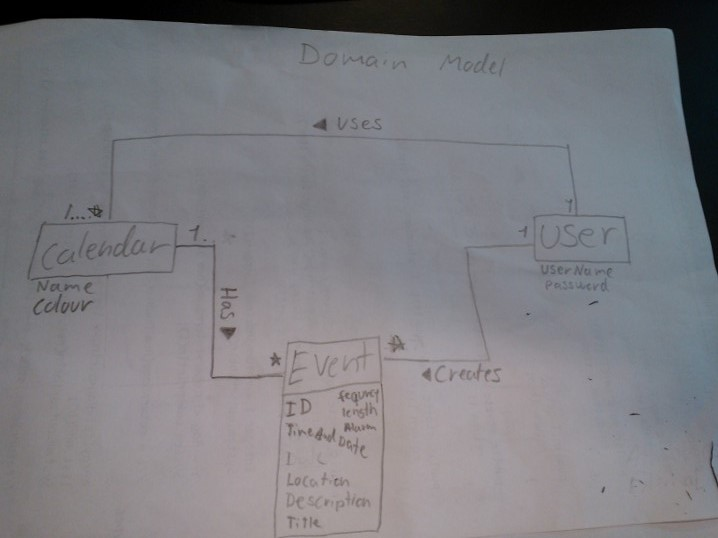
\includegraphics[scale=.65]{LatexFiles/Analyze/DomainModel/DomainModel}
   	\end{figure}
	
\newpage
	\subparagraph{System Sequence Diagram} \mbox{}

	\begin{figure}[h]
	\caption{}   
   	\hspace{-50pt}
   	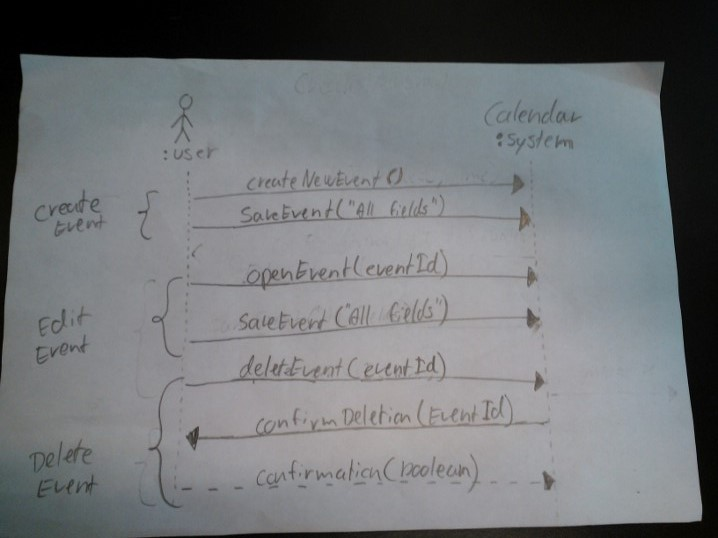
\includegraphics[scale=.65]{LatexFiles/Analyze/SystemSequenceDiagram/SSD}
   	\end{figure}

	\include*{LatexFiles/Analyze/OperationContract}   \mbox{}
	
   \paragraph{Glossary} \mbox{}
\subparagraph{Begivenhed} \mbox{}

En begivenhed repræsentere en hver form for opslag i kalenderen. Aftaler, noter, arrangementer, osv. \\
Det er kort sagt den eneste ting der kan slås op, og ses i kalenderen.


   
   \paragraph{Supplementary Requirements (FURPS+)} \mbox{}
   \subparagraph{Functionality} \mbox{}
   
   \subparagraph{Error Handling} \mbox{}
   
   In the case of a system error under the startup of the program (like no internet connection, or no calender files could be found) the user should be prompted with the question of what to do next - work offline, manually locate a calendar file or create a new calendar. \linebreak
   
   In the case of a system error when the program is running (like no internet connection), the user should also here be prompted with the question of what to do next - work offline?
   \subparagraph{Usability} \mbox{}
   
   Det skal være muligt, at anvende kalenderen uden brug af musen og kun ved hjælp af få taster.
   \subparagraph{Reliabilty} \mbox{}
   
   Kalenderen skal fungerer på en sådan måde, at den er stabil. Og hvis der skulle forekomme nedbrud, så skal kalenderen genstarte af sig selv og derved være til minimal gene for brugeren.
   \subparagraph{Performance} \mbox{}
   
   
   \subparagraph{Suportability} \mbox{}
   
   
   
   
  \end{document}
